\newpage

\chapter{Technology Stack}
This chapter will cover on technology stack needed to build the smart patch and the dashboard. It will provide an overview of what might be needed, possible technologies to choose from and choosing the most suitable ones for the development of the system.

\section{Firmware for Smart Patch}

\subsection{Computing Units - Microcontrollers (MCU)}
A microcontroller (MCU) is a compact, self-contained computer integrated on a single chip, designed for embedded applications with lightweight processing needs \cite{ref22}. MCUs are known for their small size, low power consumption, and cost-effectiveness. MCUs require a hands-on approach, involving configuration for both hardware (attachment of components, sensors, wires, etc.) and software (burning firmware, incorporating libraries, installing drivers, etc.). MCUs lack a conventional operating system and utilize firmware, a special code burned onto the device to execute specific functions and ensure proper hardware functionality. While they cannot serve as personal computers, some advanced MCUs offer features like networking, making them appealing for projects with specific requirements. \\

\begin{figure}[h!]
    \centering
    \begin{subfigure}{0.45\linewidth} % Adjust the width as needed
        \centering
        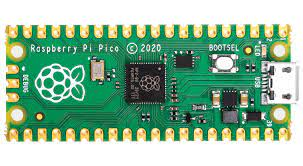
\includegraphics[width=\linewidth]{images/pico.jpg}
        \caption{Raspberry Pi Pico \cite{ref23}}
        \label{fig:pico}
    \end{subfigure}
    \hfill % This command adds space between subfigures
    \begin{subfigure}{0.45\linewidth} % Adjust the width as needed
        \centering
        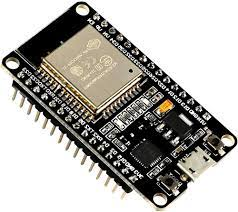
\includegraphics[width=\linewidth]{images/esp32(1).jpg}
        \caption{ESP32 \cite{ref24}}
        \label{fig:esp32}
    \end{subfigure}
    \caption{Comparison of Microcontrollers}
    \label{fig:comparison}
\end{figure}

\noindent There are multiple MCUs available in the market but the most popular ones are Raspberry Pi Pico and ESP32-WROOM-32S3-Mini-1. A comparative study between the two is provided in Table \ref{table:microcontrollers} to help in choosing the ideal MCU. \\

\begin{table}[h!]
\centering
\begin{tabularx}{\textwidth}{|X|X|X|}
\hline
\textbf{Feature} & \textbf{Raspberry Pi Pico} & \textbf{ESP32-WROOM-32S3-Mini-1} \\ \hline
Manufacture & Raspberry Pi Foundation & Espressif Systems \\ \hline
Architecture & ARM Cortex-M0+ & Xtensa LX6 \\ \hline
Processor Clock Speed & Up to 133 MHz & Up to 240 MHz \\ \hline
Wireless Connectivity & None & Wi-Fi, Bluetooth (BLE) \\ \hline
Memory & 2MB Flash (No built-in RAM) & 2MB Flash \\ \hline
GPIO Pins & 26 & Approximately 38 \\ \hline
Development Environment & MicroPython, C/C++ with Pico SDK & Arduino IDE, PlatformIO, Espressif IDF \\ \hline
\end{tabularx}
\caption{Comparative study between Raspberry Pi Pico and ESP32-WROOM-32S3-Mini-1}
\label{table:microcontrollers}
\end{table} 

\noindent Comparing the two, ESP32-WROOM-32S3-Mini-1 comes out as ideal for the Smart Patch because of its in-built wireless connectivity. It is important to have such connectivity to provide portability of the device so that wearer can wear it all day and still can go around the campus.

\noindent To power the microcontroller, we'll either provide direct power through the C-pin or utilize a LiPo battery for portability and extended use.

\subsection{Sensors}
MCUs typically come equipped with general-purpose I/O pins (GPIO), allowing users to connect various external peripherals to the computer. Examples of common input devices include sensor modules, microphones, and cameras, while output devices encompass LEDs, speakers, displays, and more. Users can program these individual pins to receive data. 

\subsubsection{Heart Rate Sensors}
To calculate HRV, heart rate sensors have to be used and connected with the MCU. Two sensors which are used abundantly in the industry, especially healthcare are ECG Sensors and Pimoroni Pulse Sensor. A comparative study is provided in Table \ref{table:heart-rate-sensor} to help in determining the ideal sensor. 

\begin{table}[p]
\centering
\begin{tabularx}{\textwidth}{|X|X|X|}
\hline
\textbf{Features} & \textbf{ECG Sensor} & \textbf{Pimoroni Pulse Sensor} \\ \hline
\textbf{Working Principle} &
ECG Sensor measures the heart's electrical activity over time \cite{ref25}. It detects the heartbeat rhythm regularly to keep a check on the health of your heart \cite{ref26}. &
Pimoroni Pulse Sensor uses a technique called photoplethysmography (PPG) to detect the change in the colour of your skin with each beat of your heart when the sensor is pressed against your fingertip \cite{ref27}. \\ \hline
\textbf{Use Cases} & 
It can detect Arrhythmias like Atrial fibrillation and can also warn you about heart attack using strokes and movements around the heart. & 
It can be used by students, artists, athletes, makers, and game \& mobile developers who want to easily incorporate live heart-rate data into their projects. \\ \hline
\textbf{Compatibility} &
Works with most smartwatches. &
Works with Arduino, micro:bit, littleBits, and most maker platforms. \\ \hline
\textbf{Intrusivity} &
Non-invasive requires skin contact. &
Less intrusive, fingertip contact. \\ \hline
\textbf{Additional Features} & 
Some devices can export an ECG graph of your heart rate, which can be a huge help when talking to your doctor. &
The Pulse Sensor has 3 holes around the outside edge which make it easy to sew it into almost anything. \\ \hline
\textbf{Image} & 
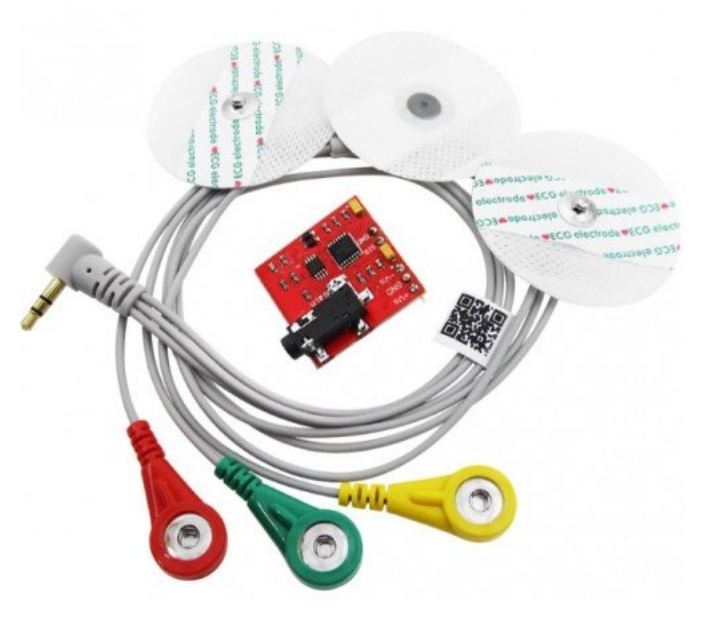
\includegraphics[width=\linewidth]{images/ecg.png}
& 
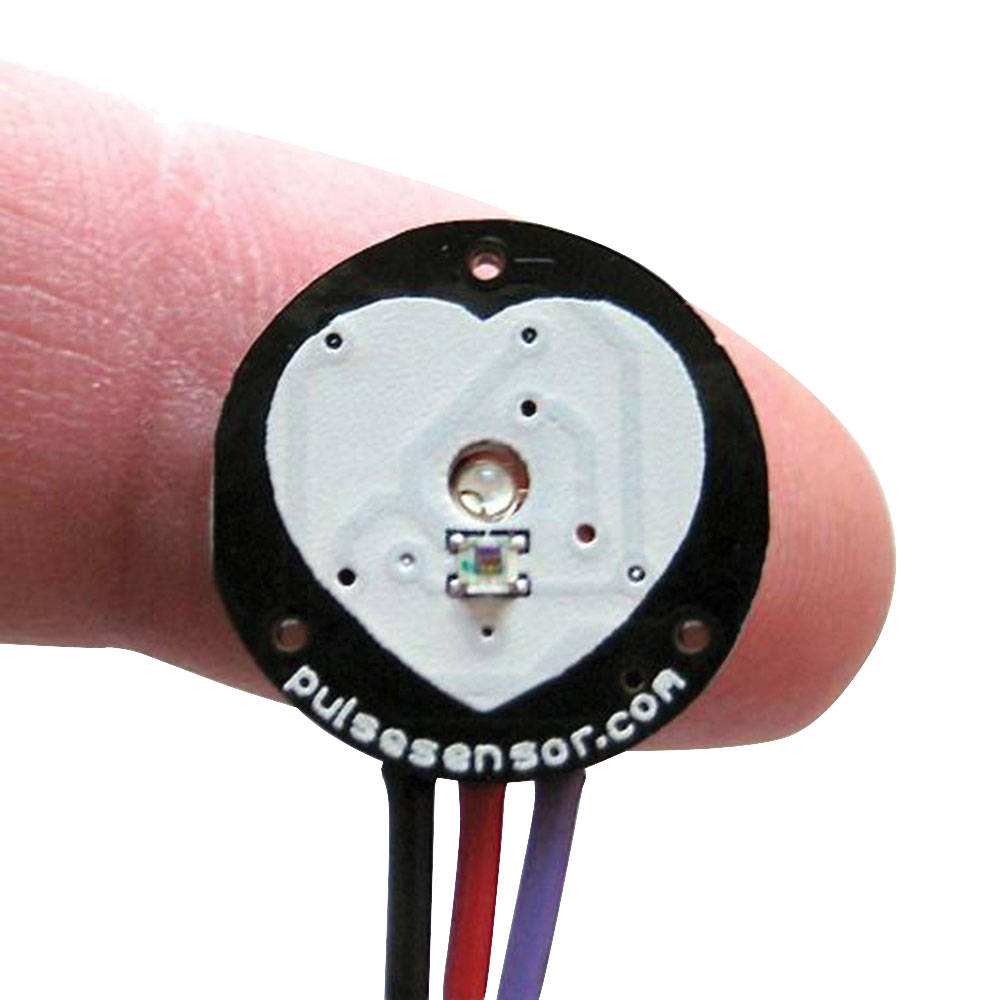
\includegraphics[width=\linewidth]{images/s75-0818p01wj.jpg}
\\ \hline

\end{tabularx}
\caption{Comparative Study between ECG Sensor and Pimoroni Pulse Sensor}
\label{table:heart-rate-sensor}
\end{table}

One of the main features of the Smart Patch is non-intrusivity. While both the sensors are efficient and used widely, Pulse Sensor comes out as a perfect choice for Smart Patch because not only it is less intrusive but also it works well with ESP32 (Arduino).

\subsubsection{Body Temperature Sensor}
% To calculate body temperature, thermometers are used normally in healthcare. But thermometers are not digital devices and therefore can’t be connected to the smart patch. Other sensors which are widely used for sensing temperature are thermistors and LM-35 sensors. Thermistors are more temperature-sensitive resistors and not sensors and require a readout circuit, which makes it harder to integrate them seamlessly into Smart Patch. On the other hand, the LM-35 Sensor is a precision IC temperature sensor. It provides a linear voltage vs temperature characteristic making it easier to figure out the temperature. It can operate over a temperature range of \(−55°C to 150°C\) and has an accuracy of \(±1\) degree Celsius. Hence, LM-35 stands out as a clear choice for this project.

\begin{figure}[!h]
    \centering
    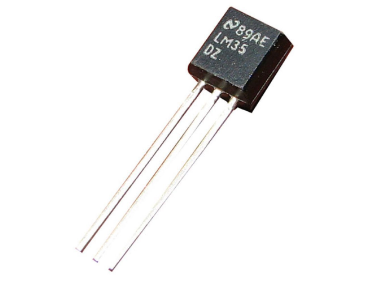
\includegraphics[width=0.25\linewidth]{images/lm-35-image.png}
    \caption{LM-35 Sensor \cite{ref28}}
    \label{fig:lm-35-sensor}
\end{figure}

\subsection{Connectivity Technology}
Connective Technology is nothing but a network of connected “smart” devices that communicate seamlessly over the internet. Wi-Fi, Bluetooth and LoRaWAN are the most used networks associated with IoT. Table \ref{table:connective-technology} provides a comparative study between the three to help in choosing the most suitable technology for the project.\\
\begin{table}[h]
    \centering
    \begin{tabularx}{\textwidth}{|X|X|X|X|}
        \hline
        \textbf{Features} & \textbf{Wi-Fi} & \textbf{Bluetooth} & \textbf{LoRaWAN} \\ \hline
        \textbf{Scalability} & Limited for massive IoT. & Mesh supports large networks. & Scales well for wide area. \\ \hline
        \textbf{Power Efficiency} &  High power consumption.& Low Energy, efficient. & Low power usage. \\ \hline
        \textbf{Range and Coverage} & Short to medium range.&Moderate, indoor range.&Long-range, wide coverage. \\ \hline
        \textbf{Data Rate} & High-speed data transfer & Moderate data rates & Low data rates \\ \hline
        \textbf{Cost and Infrastructure} & Existing infrastructure may be costly. & Cost-effective, integrated widely. & Low infrastructure cost\\ \hline
        \textbf{Security} & Robust encryption, authentication & Secure with enhancements& Implement AES encryption \\ \hline
    \end{tabularx}
    \caption{Comparative Study between Connective Technologies}
    \label{table:connective-technology}
\end{table}

\begin{figure}
        \centering
        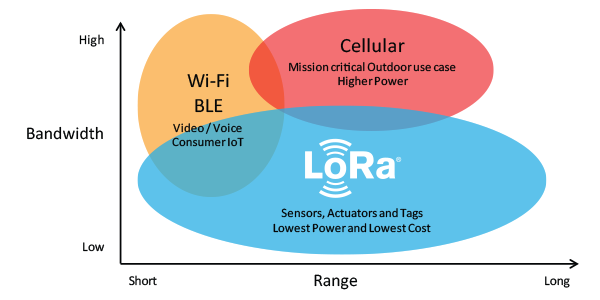
\includegraphics[width=\linewidth]{images/connective-technology.png}
        \caption{Connective Technologies compared against Bandwidth and Range \cite{ref29}}
        \label{fig:connective-technology}
    \end{figure}

From the comparison in Table \ref{table:connective-technology} and Figure \ref{fig:connective-technology}, LoRaWAN stands out as a clear and most efficient choice for Smart Patch. But the only disadvantage is that this network is not usually found in healthcare institutions compared to Wi-Fi which is available in nearly every healthcare institution. This advantage of Wi-Fi makes it easier to integrate Smart Patch with existing resources of institution thereby saving extra cost and other resources. Hence, Smart Patch will use Wi-Fi as its connective technology.

\newpage
\section{Software for Smart Patch}
\subsection{Programming Environment}
Arduino IDE, Espressif IDF (IoT Development Framework), and PlatformIO are three different programming environments used for developing software for microcontrollers and embedded systems. Each has its own strengths, weaknesses, and use cases.

\begin{table}[h]
    \centering
    \begin{tabularx}{\textwidth}{|X|X|X|X|}
        \hline
            
         & \textbf{Arduino IDE} 
         & \textbf{Espressif IDF} 
         & \textbf{PlatformIO} \\ \hline

         \textbf{Purpose} 
         & Beginner-friendly prototyping 
         & Advanced ESP32/ESP8266 development
         & Cross-platform IoT development \\ \hline

         \textbf{Language Support}
         & C/C++ with simplified syntax
         & Full C/C++ language support
         & Supports multiple languages \\ \hline

         \textbf{Hardware Compatibility}
         & Extensive hardware compatibility
         & Specifically for ESP32/ESP8266 
         & Broad hardware support \\ \hline

         \textbf{Integration}
         & Integrated Development Environment
         & Integrated toolchain for ESP 
         & Integrated platform and library manager \\ \hline
    
    \end{tabularx}
    \caption{Comparative Study between Programming Environments}
    \label{table:programming-environment}
\end{table}

For the project, Arduino IDE emerges as the preferred choice after comparing the three environments (as outlined in Table \ref{table:programming-environment}). Its beginner-friendly nature suits the project's prototyping needs, and it offers extensive hardware compatibility. Additionally, Arduino IDE's simplified syntax aligns well with the project's requirements.

\subsection{Programming Languages}
ESP32 is compatible with 2 programming languages - Arduino C++ and MicroPython. Both of these languages are popular and used widely to program the firmware. The table \ref{table:programming-language} provides features of each of these languages.

\begin{table}[h]
    \centering
    \begin{tabularx}{\textwidth}{|X|X|X|}
        \hline

        \textbf{Features}
         & \textbf{Arduino C++}
         & \textbf{MicroPython} \\ \hline

        \textbf{Use} 
        & Firmware
        & Firmware \\ \hline

        \textbf{Programming Language}
        & Low-level language with simplified syntax.
        & Python optimized for microcontrollers. \\ \hline

        \textbf{Abstraction level}
        & Provides abstraction for hardware complexities.
        & Abstracts hardware with clean Python code. \\ \hline

        \textbf{Ease of Use}
        & Beginner-friendly with a simplified structure.
        & Beginner-friendly, less complex than C/C++. \\ \hline

        \textbf{Memory Usage}
        & Generally efficient memory usage. 
        & May use more memory compared to C/C++. \\ \hline

        \textbf{Application Scope}
        & Ideal for firmware development in embedded systems.
        & Suited for microcontroller programming. \\ \hline

        \textbf{Ecosystem}
        & Rich ecosystem, extensive libraries.
        & Growing ecosystem for microcontrollers. \\ \hline

        \textbf{Concurrency Model}
        & Sequential execution with setup() and loop().
        & Supports concurrency but less efficiently. \\ \hline

        \textbf{Frameworks}
        & Arduino framework for embedded systems.
        & Limited frameworks for microcontrollers. \\ \hline

        \textbf{Resource Efficiency}
        & Generally efficient in resource usage.
        & May consume more resources. \\ \hline
         
    \end{tabularx}
    \caption{Comparative Study between Arduino C++ and MicroPython}
    \label{table:programming-language}
\end{table}

\noindent Both programming languages demonstrate efficiency in their respective ways.  To determine the most suitable choice for the project, a decision matrix is employed (shown in Table \ref{fig:decision-matrix}). Each crucial feature is assessed for both languages, assigning a weighted score to each feature. Both scores and weights are provided in a range of 1 to 5.

% \begin{figure}
%     \centering
%     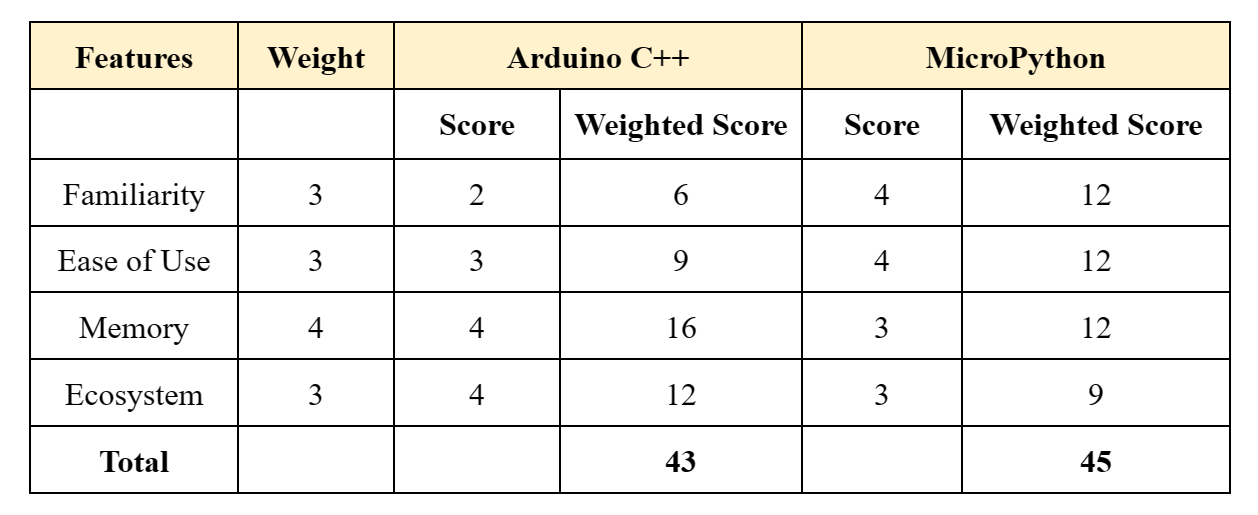
\includegraphics[width=1\linewidth]{images/decision-matrix.png}
%     \caption{Decision Matrix for Programming Languages}
%     \label{tab:decision-matrix}
% \end{figure}

\begin{table}[!h]
\centering
\begin{tabularx}{\textwidth}{|X|X|X|X|X|X|}
    \hline
    \textbf{Features} 
    & \textbf{Weight}
    & \multicolumn{2}{c|}{\textbf{Arduino C++}}
    &  \multicolumn{2}{c|}{\textbf{MicroPython}}  \\ \hline

    &
    & Score 
    & Weighted Score
    & Score 
    & Weighted Score \\ \hline

    Familiarity 
    & 3 
    & 2 
    & 6
    & 3
    & 9 \\ \hline
    
    Ease of Use
    & 3 
    & 3 
    & 9
    & 4 
    & 12 \\ \hline
    
    Memory 
    & 4 
    & 4 
    & 16
    & 3 
    & 12 \\ \hline
    
    Ecosystem 
    & 3 
    & 4 
    & 12
    & 3 
    & 9 \\ \hline
    
    \textbf{Total} 
    & 
    &
    & \textbf{43} 
    &  
    & \textbf{42}  \\ \hline
    
\end{tabularx}
\caption{Decision Matrix for Programming Languages}
\label{fig:decision-matrix}
\end{table}

\noindent Following the completion of the decision matrix, it is determined that Arduino C++ emerges as the more fitting choice of programming language for the project. \\

Alternatively, a variety of IoT solutions are accessible in the market and offered at no cost. These options span from frameworks for creating dashboards to robust cloud platforms specifically designed for IoT applications. (see \textbf{Appendix E})\\

\section{Software for Web Dashboard}
The dashboard would be nothing but a website made using HTML, CSS and Javascript (JS). The programming environment of choice will be Visual Studio Code (VSCode), providing a robust platform for web development. \\

\noindent The Flask framework will be utilized for developing the backend framework of the web dashboard. Flask is a lightweight and flexible micro-framework for Python. It offers simplicity and ease of use, making it suitable for building web applications. \\ \\
Additionally, a mixture of SQLite (for testing) and MySQL (for production) databases will be employed to manage data storage and retrieval efficiently. 
\begin{enumerate}
    \item SQLite offers a lightweight and self-contained database solution, ideal for testing and development environments. Its simplicity and zero-configuration setup streamline the process of data storage and retrieval during development.
    \item MySQL is a robust relational database management system, is well-suited for production environments due to its scalability, performance, and reliability. It provides advanced features for managing large datasets and ensuring data integrity for the web dashboard in a production setting.
\end{enumerate}

\section{Messaging API: Twilio API}
The Twilio API provides a robust platform for integrating messaging capabilities into IoT Devices. With Twilio, developers can send and receive SMS, MMS, and even WhatsApp messages programmatically, enabling real-time communication with users. Twilio API offers versatile messaging channels, global coverage, developer-friendly API, scalability, reliability, and security. This makes it the ideal choice for integrating seamless and efficient communication capabilities into the web dashboard.

\noindent Within the project scope, a thorough examination of potential risks has been undertaken, delineating possible difficulties that might emerge throughout the project’s duration. The risk register will be reviewed regularly throughout the project, allowing for the timely incorporation of newly recognised risks and fostering a proactive approach to risk management.  The primary emphasis of this section is on identifying major potential risks and devising strategies to minimise their effects. \textbf{Appendix F} provides the risk register used for the project.

